\section{Evaluation} \label{evaluation} 
To evaluate our continuous training approach, we perform several experiments.
We first describe the setup of our experiments including the computing cluster, the deployed pipeline, and how we simulated a real production environment by streaming a real-world large dataset through our deployment platform.
First, we discuss the effect of different parameters (learning rate adaptation, sampling strategy, and scheduling rate) on the quality and training time of the model.
Then, we discuss the effects of proactive training on the quality of the model and compare it to the quality of a model that is trained on a daily basis.
Finally, we evaluate the effects of online statistics computation and data materialization optimizations on the training time.

\subsection{Setup}\label{subsec:setup}
We evaluate our deployment method in distributed environment consists of 21 nodes (1 master, 20 slaves).
Each node is running on an Intel Xeon 2.40 GHz 16 core processor and has 28 GB of dedicated memory for running our prototype.

To demonstrate the deployment platform designed the following machine learning pipeline.

\textbf{Criteo Pipeline.} 
The Criteo pipeline consists of 5 operations: input parser, missing value imputer, standard scaler, one hot encoder, and logistic regression model trainer. 
The Terabyte Criteo click log dataset is used for benchmarking algorithms for clickthrough rate (CTR) prediction \cite{criteo-log}.
It contains 24 days of user click logs. 
The dataset  contains 13 numerical and 26 categorical features. 
In all of our experiments we are using the data from the first 6 days (Day 0 to Day 5) of the Criteo dataset.
Day 0 is used for the initial offline training of the pipeline.
Day 1 to Day 5 are used as a streaming dataset.
To evaluate the quality of the pipeline, we use a sample of the Day 6 to compute the logistic loss.

\textbf{Criteo Data Simulation.}
We simulate a production environment by streaming 5 days of criteo dataset.
The data from each day is divided into 1440 smaller batches and stored on disk.
Each batch represent one minute of data.
We use spark streaming to read the data files one by one and stream them through the deployment platform. 

\subsection{Learning Rate Adaptation Method}
In Section \ref{sgd}, we discussed the importance of learning rate tuning for training a model using the Stochastic Gradient Descent optimization method.
Proactive training is an extension of SGD, therefore the process of tuning the learning rate adaptation method is no different from tuning the it for a normal offline SGD training.

Figure \ref{fig:criteo-learning-rate} shows the log loss for different learning adaptation methods. 
During the training phase, we evaluated the logistic loss on evaluation dataset after 20, 40, 80, 160, 320, and 500 iterations.
Both Adadelta and Momentum performs very poorly on the criteo data.
Criteo dataset is a complex and high dimensional dataset, where features are a mix of numerical and categorical.
Since categorical features are not standardized, Adadelta and Momentum are not able to effectively tune the learning rate for a mix standardized and non-standardized features.
Both RMSPROP and ADAM manage to effectively reduce the logistic loss during the training phase.
Both methods resulted in the model to converge after 500 iterations.
However, ADAM achieves a lower error rate on the evaluation data when compared to RMSPROP.
After 500 iterations of training, we deploy the pipelines.
We streamed Day 1 of the Criteo dataset to the deployment system and monitored the changes in the loss using the same evaluation dataset.
After deployment, both RMSPROP and Adam further decreased the loss from 0.190 and 0.155 to 0.185 and 0.151 respectively.
Adadelta also reduces the loss by around 0.004, however, the deployed pipeline trained using Adadelta learning rate adaptation technique was not fully converged and as a result the final error rate after the first day is still quite high.
For the rest of our experiments, we chose ADAM as the learning rate adaptation technique.
When using ADAM, the model converges using fewer number of iterations as compared to other learning rate adaptation methods.
Moreover, ADAM is the most effective learning rate for continuous training of the pipeline as well.

This experiment shows that choosing learning rate adaption technique for proactive training is similar to choosing the learning rate adaptation technique for offline SGD.
This indicates that while ADAM is the best learning rate adaptation technique for Criteo pipeline, it is not necessarily the best for other pipelines and datasets.
For every pipeline and dataset, the users have to evaluate the performance of the different learning rate adaptation techniques during the offline training of the model and chose the best method for both offline and proactive training of the model.


\begin{figure}[h!]
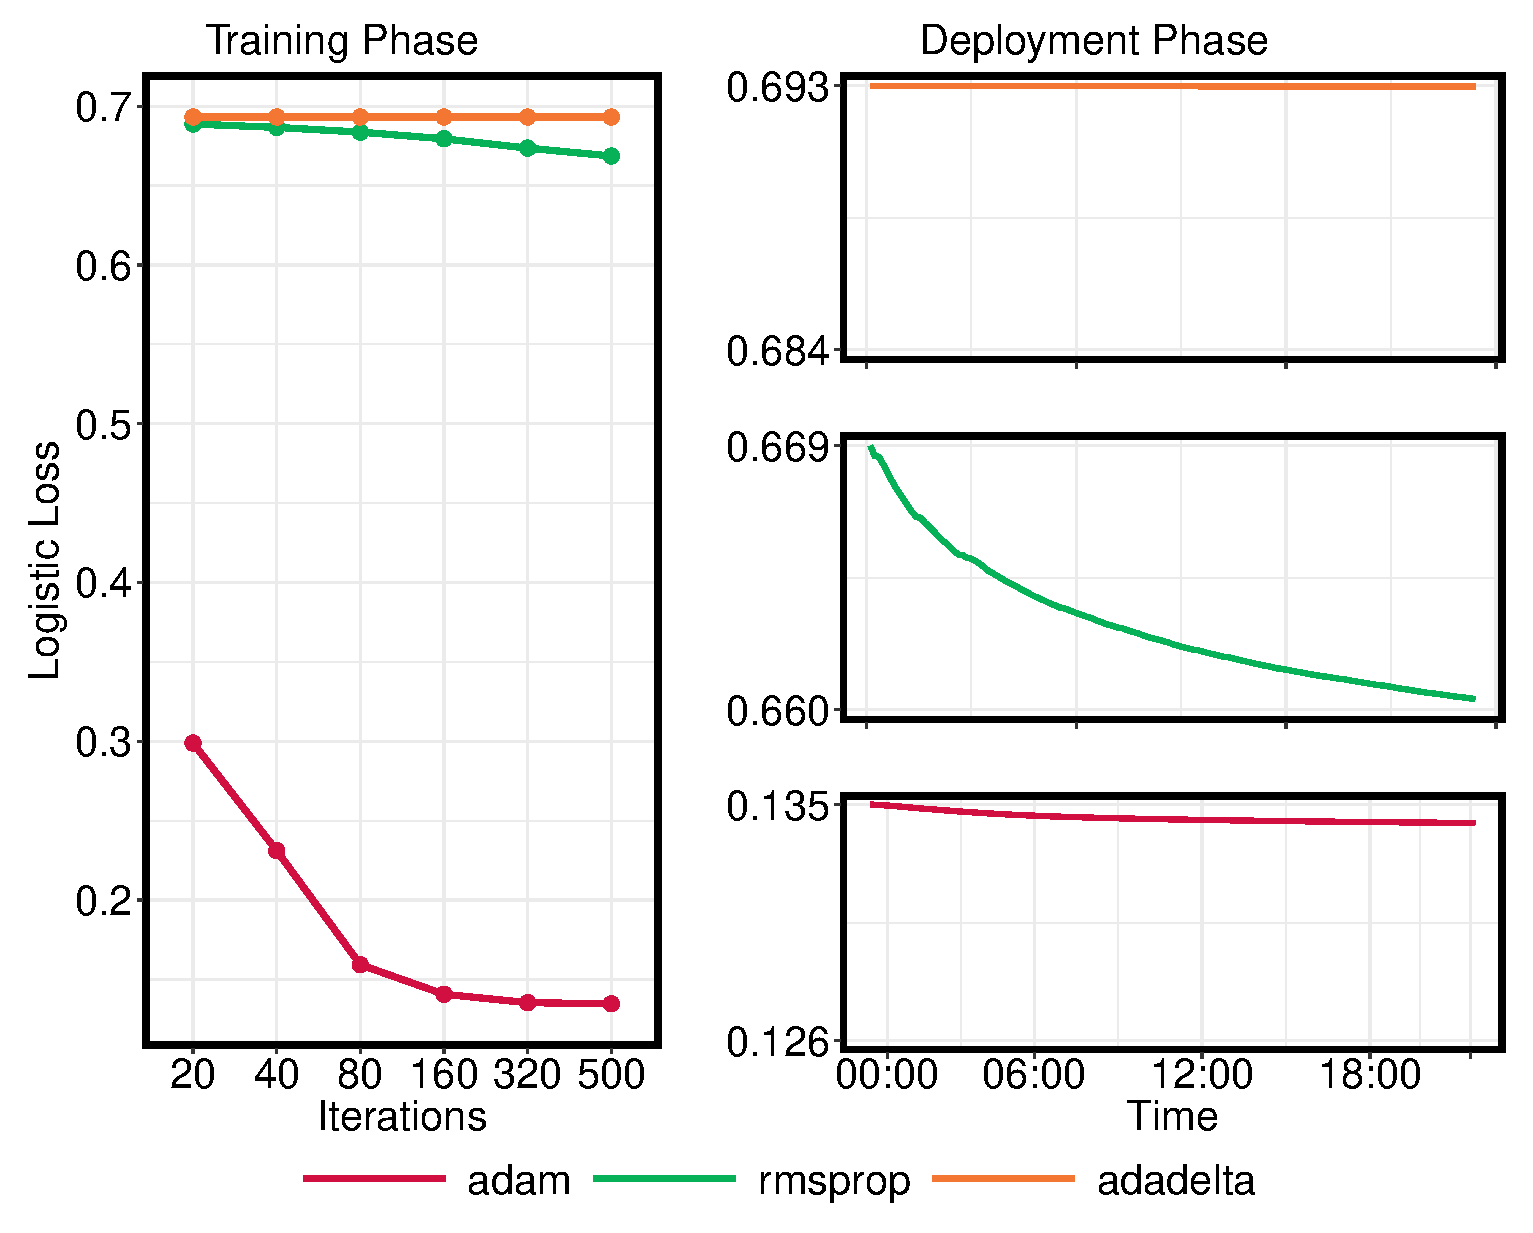
\includegraphics[width=\columnwidth]{../images/experiment-results/criteo-learning-rate-experiment.eps}
\caption{Learning rate adaptation technique for Criteo pipeline}
\label{fig:criteo-learning-rate}
\end{figure}

\subsection{Sampling Methods}
In this section, we discuss the effects of different sampling modes on the quality of the deployed model.
Figure \ref{fig:sampling-mode-quality} shows how different sampling approaches during the continuous training of the Criteo pipeline affects the logistic loss error rate.
Different windows sizes affect the stability of the model quality.
For experiments using a sampling window size (entire history, one day, and half a day), first the data is sampled and then the new training data that arrived at the system recently is appended to the sample and used in proactive training.
Using the entire historical data to make the samples for proactive training results in a logistic error rate that decreases in a steady manner over time.
However, the error rate of the model after 5 days of continuous training is larger than other sampling approaches.
Using a limited sampling window size reduces the error rate when compared to sampling the entire historical data, however, the error rate is slightly unstable.
A larger window size (1 day) results in a more stable error rate and after 5 days of continuous training achieves the lowest error rate when compared with all the other methods.
When sampling is switched off (window size equals to zero), the error rate is unstable and it sometimes fluctuates by a margin of 0.1.
When no sample of the historical data is used, the model is only trained using new data, therefore, the changes in the model weight are much larger.
During the first 3 days of continuous training, the model trained with sampling switched off, results in the lower error rate.
However, after the 4th of training, the error rate goes up.

This experiment shows that the sampling window size affects both the stability and the error rate of the model.
Larger sampling window sizes, increase the stability of the window at the expense of slower convergence. 
Smaller sampling window sizes, decrease the error rate, however, the error rate is not stable and with every proactive training, the error rate may slightly go up.
We use a window size of one day for the rest of our experiments as it leads to a low and stable error rate throughout the deployment process.


\begin{figure}[h!]
\centering
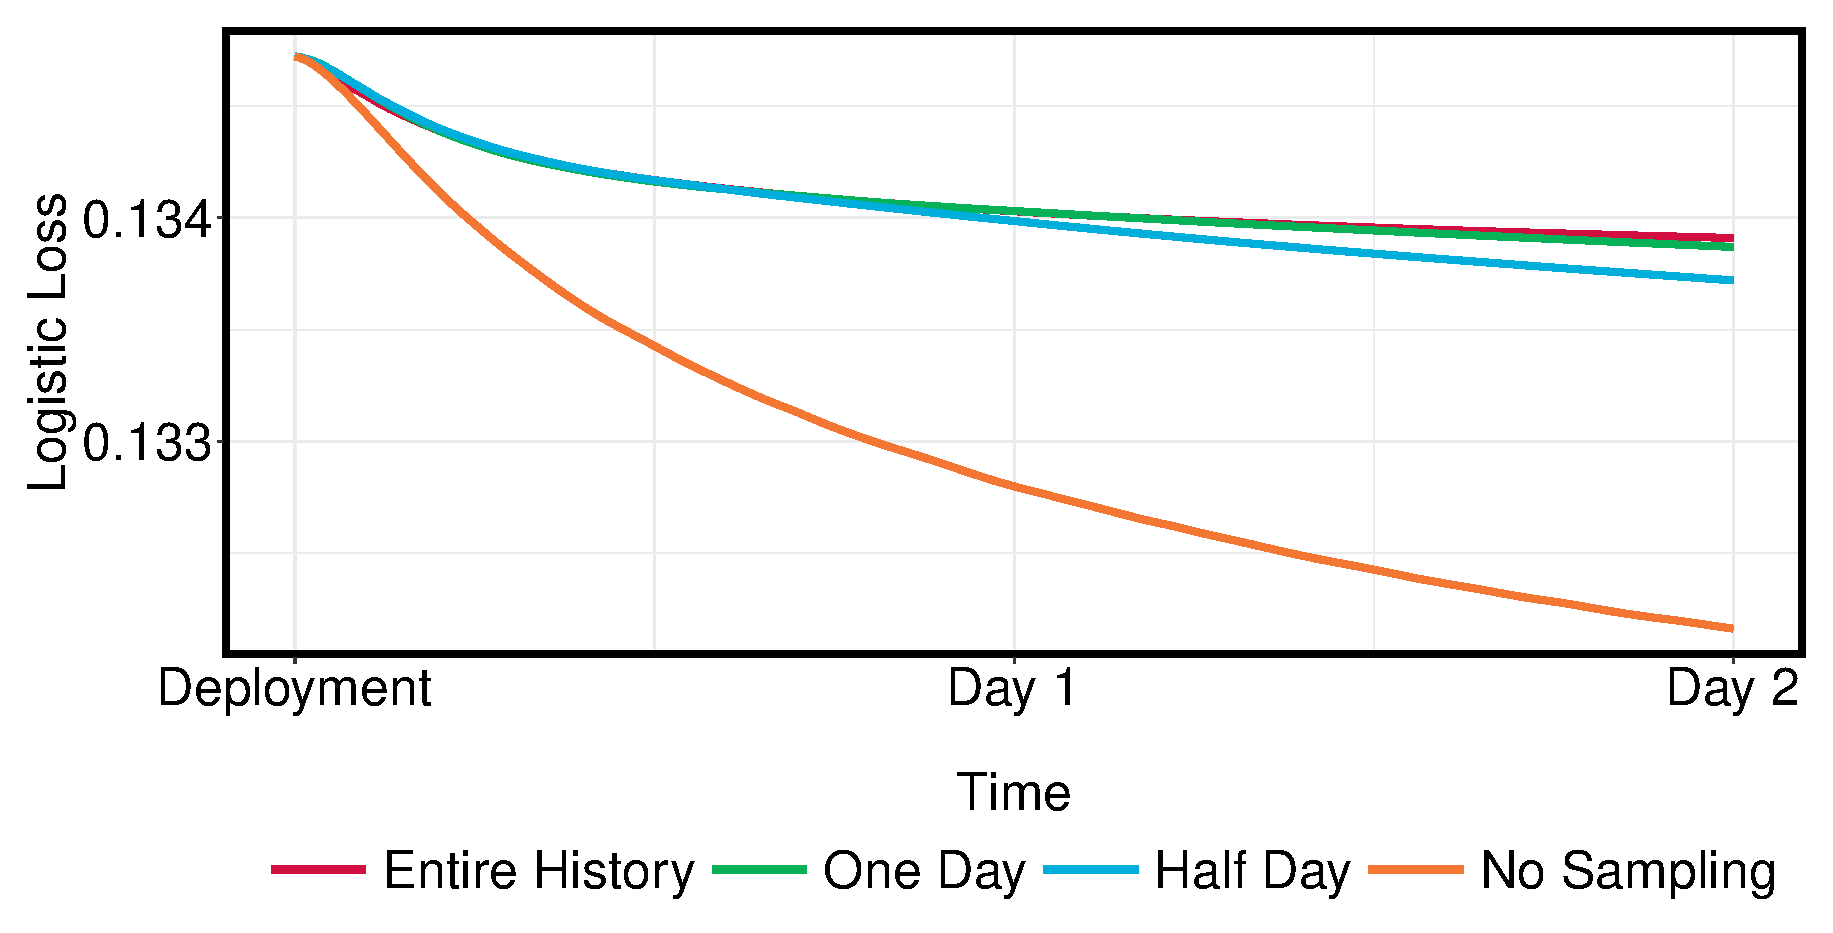
\includegraphics[width=\columnwidth]{../images/experiment-results/criteo-sampling-mode-experiments.eps}
\caption{Effect of different sampling modes on quality}
\label{fig:sampling-mode-quality}
\vspace{2mm}
\end{figure}

\begin{figure}[h!]
\centering

\includegraphics[width=\columnwidth]{../images/placeholder.jpeg}
\caption{Effect of Sampling mode on time}
\label{fig:sampling-mode-time}
\vspace{2mm}
\end{figure}



\subsection{Scheduling Policy}
In this section I will investigate the effect of different scheduling rate.
From the simulation I will check the quality for 10 minute and one hour interval and compare the quality to the daily training.
Then I will use the formula in chapter 3 to do the scheduling and compare the quality of the model using that approach.

\begin{figure}[h!]
\centering

\includegraphics[width=\columnwidth]{../images/placeholder.jpeg}
\caption{Effect of Scheduling rate on quality (10 minutes, 1 hour, automatic)}
\label{fig:scheduling-policy-quality}
\vspace{2mm}
\end{figure}

\begin{figure}[h!]
\centering

\includegraphics[width=\columnwidth]{../images/placeholder.jpeg}
\caption{Effect of Scheduling rate on training time (10 minutes, 1 hour, automatic)}
\label{fig:scheduling-policy-time}
\vspace{2mm}
\end{figure}


\subsection{Proactive Training}
I this section the quality of the model trained using proactive and daily are compared.
\begin{figure}[h!]
\centering
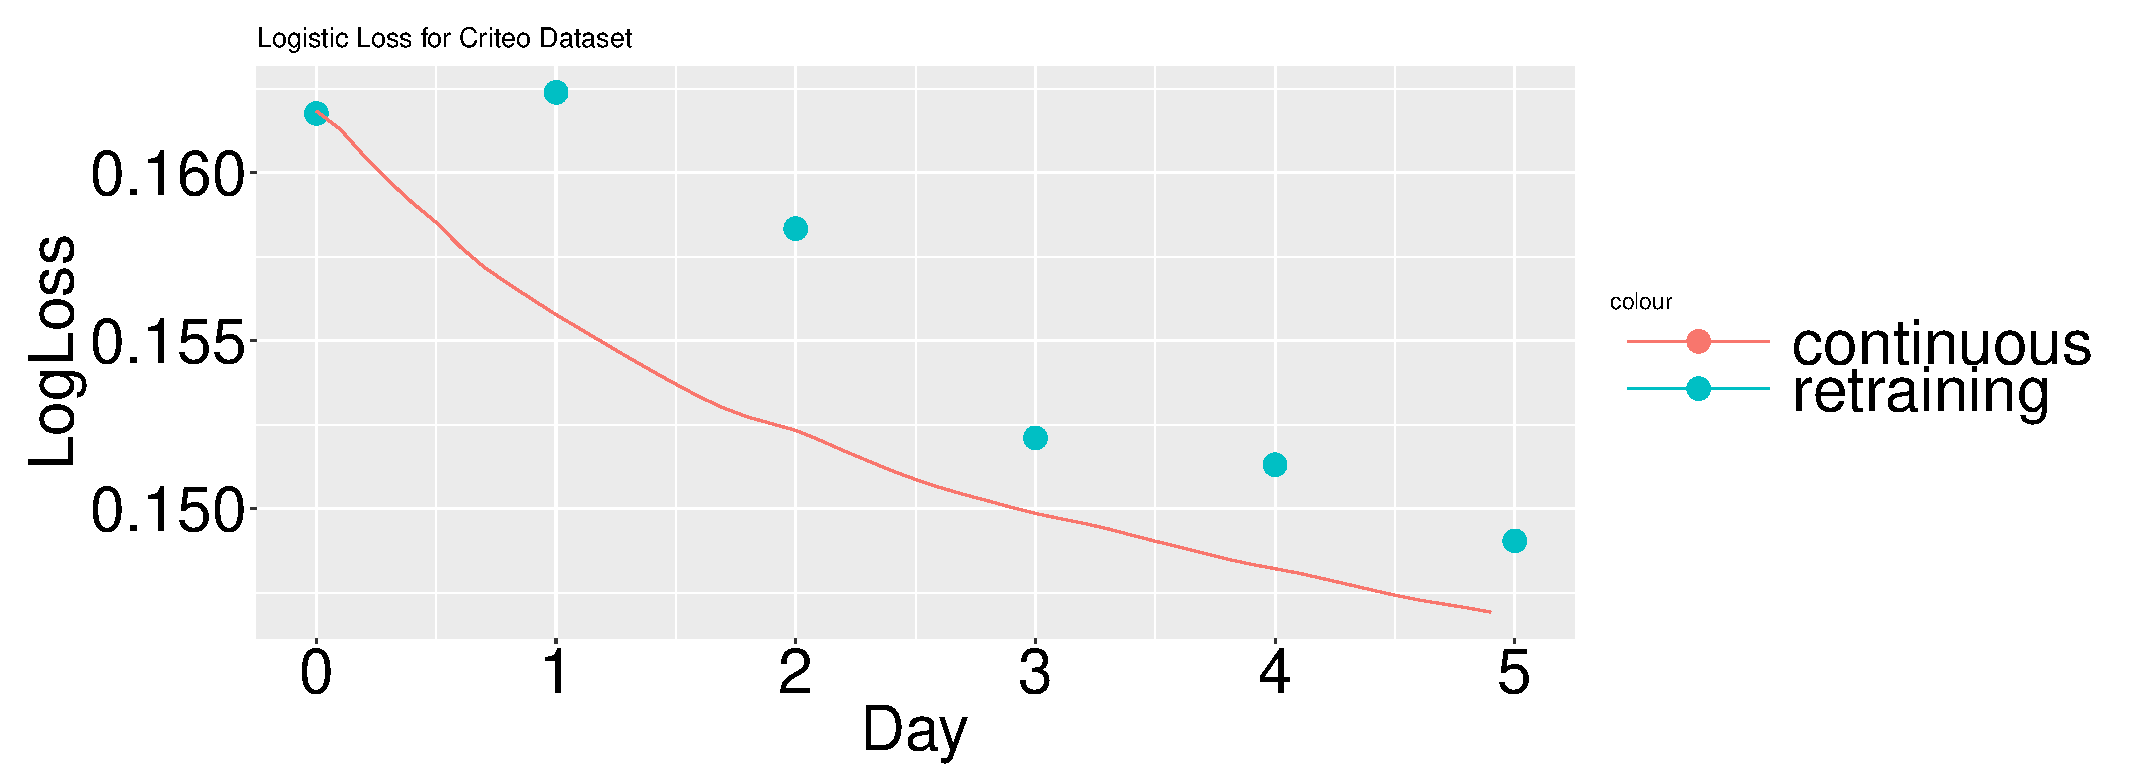
\includegraphics[width=\columnwidth]{../images/experiment-results/criteo-log-loss-continuous-vs-daily.eps}
\caption{Total training time of the pipeline for each scenario}
\label{fig:loss-proactive-vs-daily}
\vspace{2mm}
\end{figure}


\subsection{Model Freshness}
We measure model freshness by two metrics: training recency and rate of new features.
Training recency is determined by the scheduling rate.
Performing more frequent training results in models that can adapt to changes in the data more rapidly.
In Criteo pipeline, we use a feature encoder to transform the categorical features into binary indicator variables.
The initial training data (Day 0) only contains a small portion of all the unique categorical features of the Criteo dataset.
The incoming training data may contain features that have not existed in the dataset before.
Figure \ref{fig:criteo-feature-discovery} shows the feature size over time for the first 5 days after deployment of Criteo pipeline.
The rate of incoming new features is roughly 30,000 per minute and every day around 45 million new features are generated.

Using our continuous training approach, we update the pipeline as soon as new features become available.
During the next scheduled proactive training, the model is updated using these new features.
As a result, the deployed pipeline is able to answer prediction queries that may contain the same set of features more accurately.
Using a daily training approach, any unseen features that arrive at the system are dropped before a prediction is made.

\begin{figure}[H]
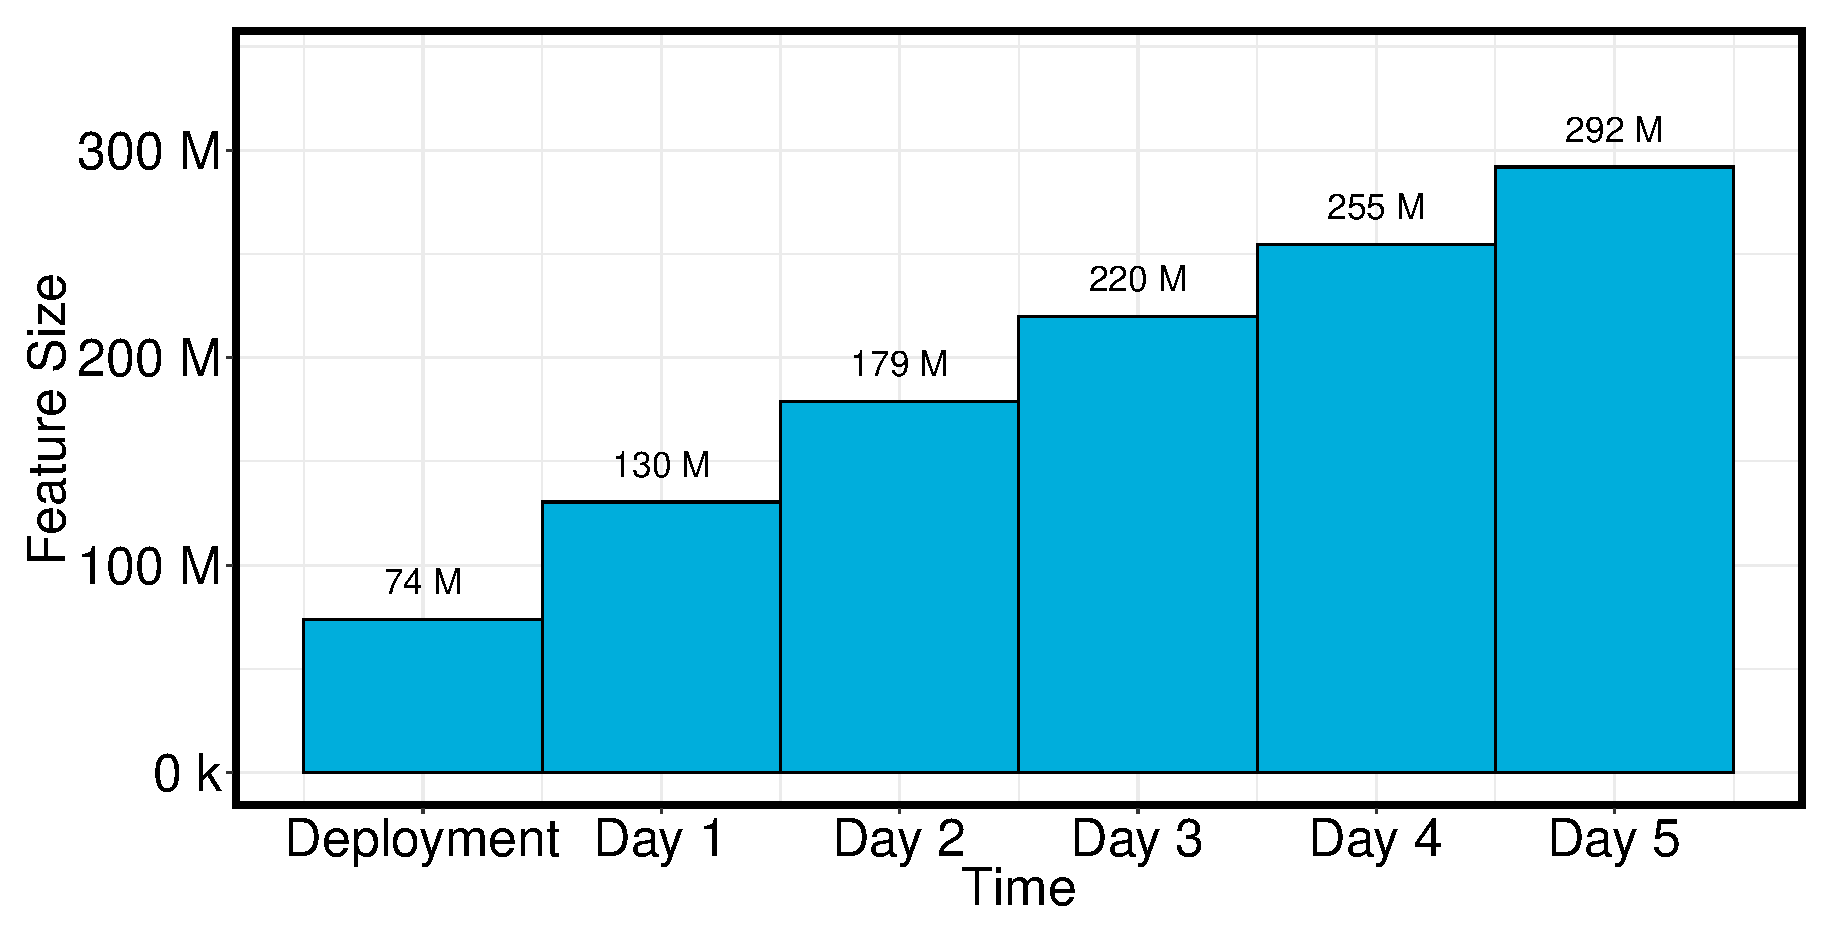
\includegraphics[width=\columnwidth]{../images/experiment-results/criteo-feature-discovery-experiment.eps}
\caption{Criteo categorical feature size over time}
\label{fig:criteo-feature-discovery}
\end{figure}



\subsection{Total Training Time}
In this section, the total training time for continuous and periodical deployment approaches are measured.
The total training time includes the time spent in pre-processing the training and model training.
Figure \ref{fig:training-time-deployment} shows the total time the deployment platform spends in training the Criteo pipeline for different deployment approaches.
Using continuous training, the time spent in training is almost a third of periodical training.
This is due to the large of amount of redundant data processing and model training that exists in periodical deployment approach.
In periodical deployment, the underlying pipeline is trained from scratch every day, which includes ingesting the data stored on disk, performing the data transformation steps of the pipeline and finally training the model using the transformed data.
However, in continuous training, the pipeline is incrementally updated when new data arrives at the system.
Moreover, the total training time can be further reduced in the continuous training approach by switching on the online statistics update and materialization optimizations.
Figure \ref{fig:training-time-optimization} shows the effect each optimizations on the continuous training approach.
Using materialized data, the total training time is furthered reduced by a factor of 3.
Using statistics update and materialization enables us to process and materialize the data and update the pipeline components in real-time.
As a result, proactive training accesses the materialized data and can directly train the model and skip the data transformation steps of the pipeline.

\begin{figure}[h]
\begin{subfigure}{\columnwidth}
\centering
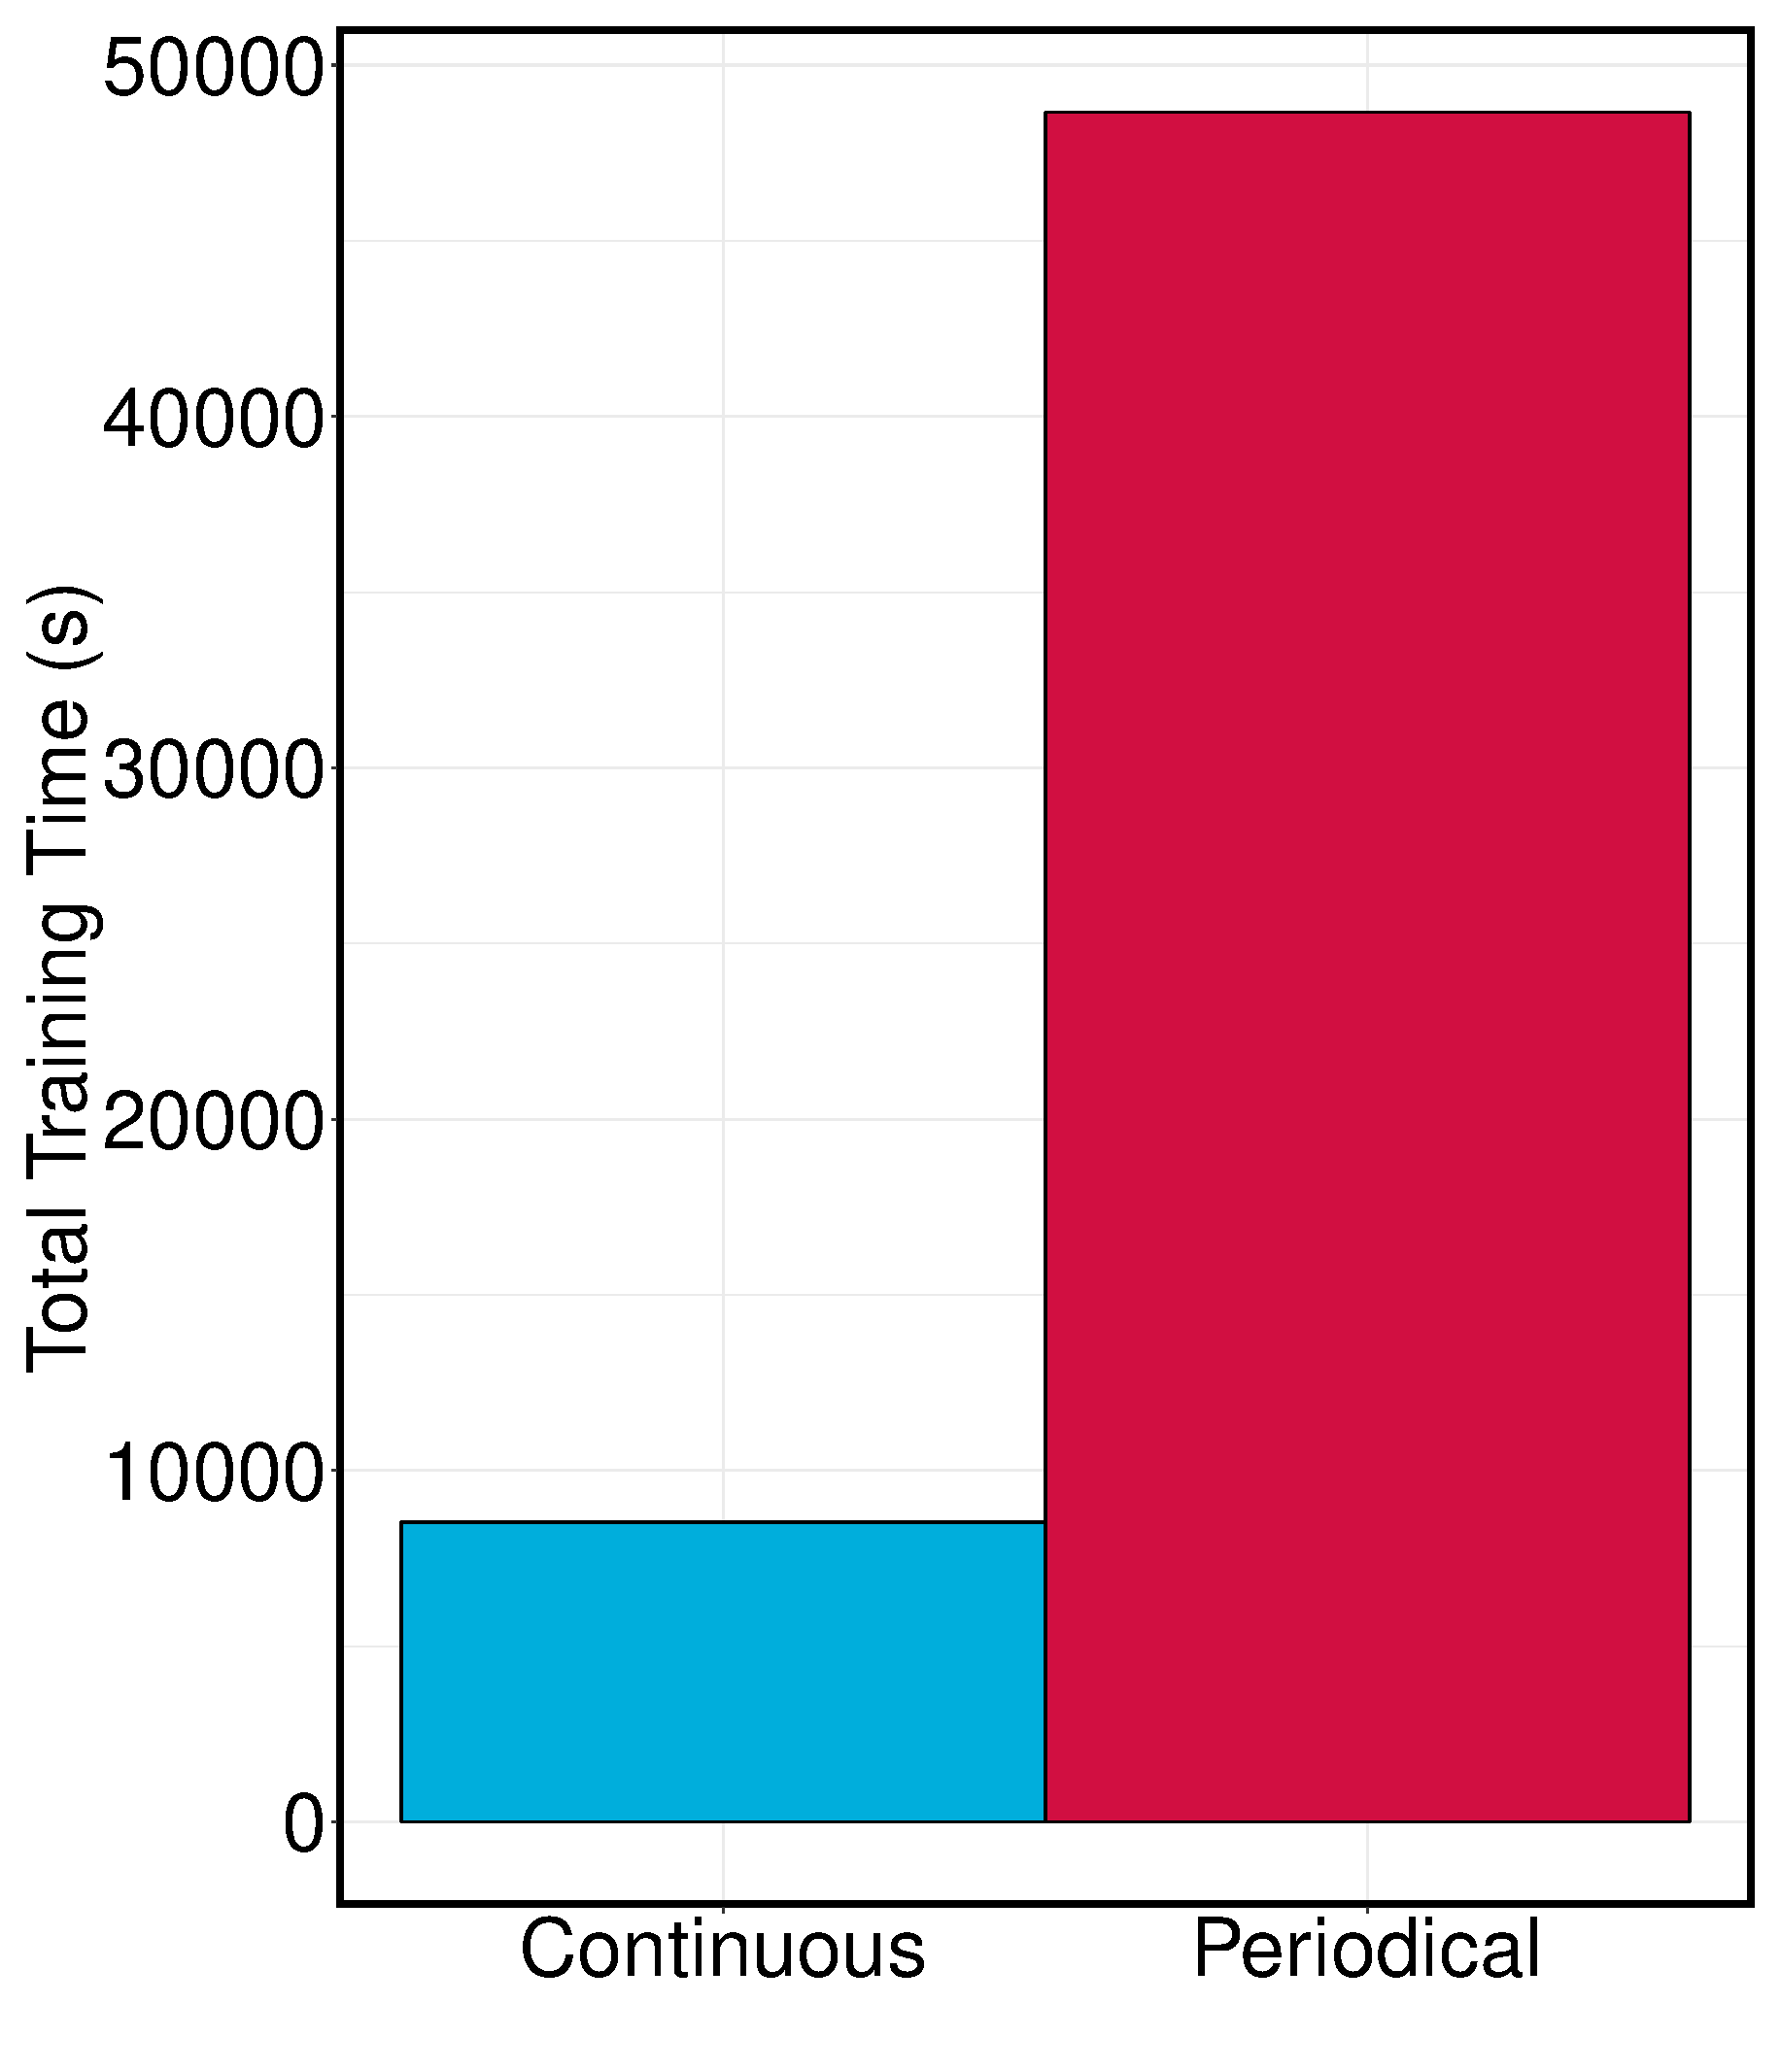
\includegraphics[width=\columnwidth]{../images/experiment-results/criteo-training-time-deployment-types-experiment.eps}
\caption{Deployment Approaches}
\label{fig:training-time-deployment}
\end{subfigure}
\begin{subfigure}{\columnwidth}
\centering
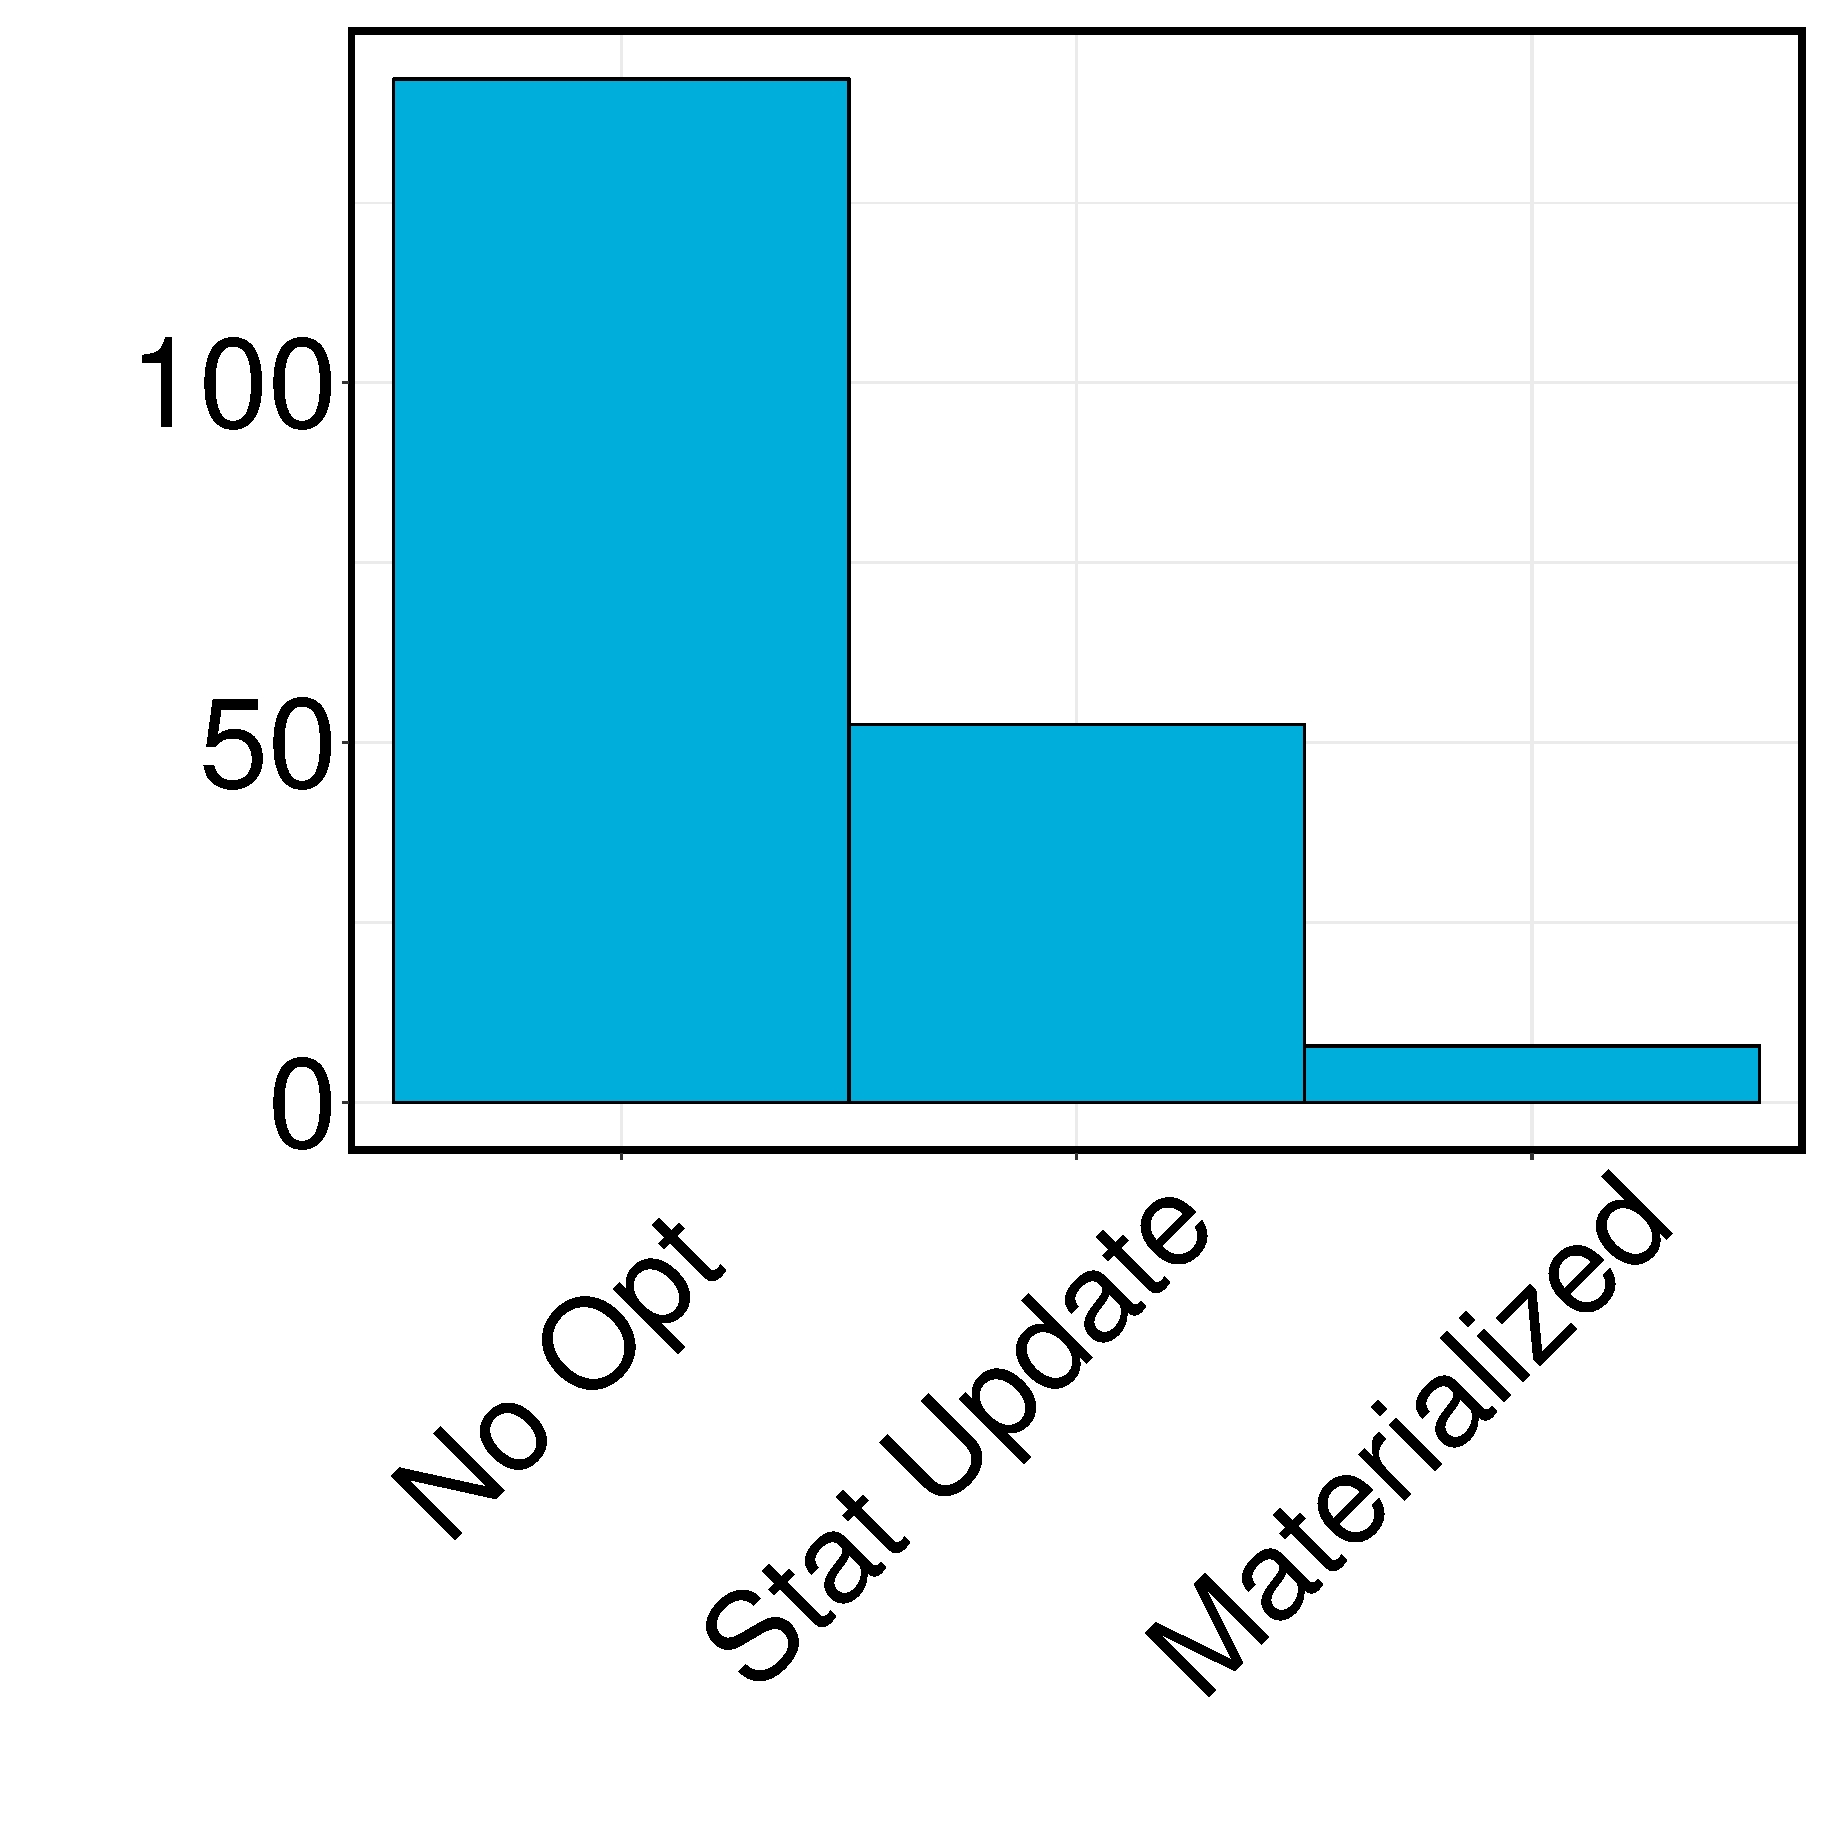
\includegraphics[width=\columnwidth]{../images/experiment-results/criteo-training-time-optimizations-experiment.eps}
\caption{Optimizations}
\label{fig:training-time-optimization}
\end{subfigure}
\vspace{2mm}
\caption{Total training time for different deployment approaches (with optimizations enabled)}
\end{figure}

One possible problem with the materialization optimization is the amount of space required to store the materialized dataset.
Depending on the type of the data processing the size of the materialized data may increase.
In our experiments, after processing the data using the Criteo pipeline the size of the materialized data increased by a factor of 2.
Therefore, the users of the system have to ensure that the space requirement of the system is met before turning on the materialization optimization.

\subsection{Discussion} \label{subsec:discussion}
discussion of the results
